\documentclass[aspectratio=169,11pt]{beamer}

% ---------- Theme ----------
\usetheme[numbering=fraction]{metropolis} % clean modern theme
\setbeamertemplate{caption}{\raggedright\insertcaption\par}

% ---------- Packages ----------
\usepackage[T1]{fontenc}
\usepackage{lmodern}
\usepackage{amsmath,amssymb}
\usepackage{booktabs}
\usepackage{graphicx}
\usepackage{multicol}
\usepackage{hyperref}
\usepackage{caption}

% (Optional) speaker notes
% \usepackage{pgfpages}
% \setbeameroption{show notes on second screen=right}

% ---------- Metadata ----------
\title{Model Compression and Efficiency Optimisation\\for Edge Deployment}
\subtitle{Diploma Seminar 1 --- Introduction and Literature Review}
\author{Hubert Jaczyński}
\institute{
  Warsaw University of Technology\\
  \vspace{1mm}
  \footnotesize Supervisor: PhD. Maria Ganzha
}
\date{Warsaw, 2026}

% ---------- Helpers ----------
\newcommand{\noteTime}[1]{\note{\textbf{Timing:} #1}}
\newcommand{\smallurl}[1]{{\footnotesize\texttt{#1}}}

% ---------- Single-file bibliography (optional) ----------
\begin{filecontents*}{refs.bib}
@article{lecun2015deep,
  title={Deep learning},
  author={LeCun, Yann and Bengio, Yoshua and Hinton, Geoffrey},
  journal={Nature},
  volume={521},
  number={7553},
  pages={436--444},
  year={2015}
}
@inproceedings{vaswani2017attention,
  title={Attention is all you need},
  author={Vaswani, Ashish and Shazeer, Noam and Parmar, Niki and others},
  booktitle={NeurIPS},
  year={2017}
}
@inproceedings{dosovitskiy2021vit,
  title={An image is worth 16x16 words: Transformers for image recognition at scale},
  author={Dosovitskiy, Alexey and Beyer, Lucas and Kolesnikov, Alexander and others},
  booktitle={ICLR},
  year={2021}
}
@article{cheng2017compression,
  title={A survey of model compression and acceleration for deep neural networks},
  author={Cheng, Yu and Wang, Duo and Zhou, Pan and Zhang, Tao},
  journal={arXiv:1710.09282},
  year={2017}
}
@article{gholami2021quant,
  title={A survey of quantization methods for efficient neural network inference},
  author={Gholami, Amir and Kim, Sehoon and Dong, Zhen and others},
  journal={arXiv:2103.13630},
  year={2021}
}
@inproceedings{han2016deepcompression,
  title={Deep compression: Compressing deep neural networks with pruning, trained quantization and huffman coding},
  author={Han, Song and Mao, Huizi and Dally, William J.},
  booktitle={ICLR},
  year={2016}
}
@article{hinton2015distill,
  title={Distilling the knowledge in a neural network},
  author={Hinton, Geoffrey and Vinyals, Oriol and Dean, Jeff},
  journal={arXiv:1503.02531},
  year={2015}
}
@inproceedings{cai2019proxylessnas,
  title={ProxylessNAS: Direct neural architecture search on target task and hardware},
  author={Cai, Han and Zhu, Ligeng and Han, Song},
  booktitle={ICLR},
  year={2019}
}
@article{sze2017efficient,
  title={Efficient processing of deep neural networks: A tutorial and survey},
  author={Sze, Vivienne and Chen, Yu-Hsin and Yang, Tien-Ju and Emer, Joel},
  journal={arXiv:1703.09039},
  year={2017}
}
@incollection{Abid2022EdgeDevices,
  author    = {Abid, Areeba and Sinha, Priyanshu and Harpale, Aishwarya and Gichoya, Judy and Purkayastha, Saptarshi},
  title     = {Optimizing Medical Image Classification Models for Edge Devices},
  booktitle = {Distributed Computing and Artificial Intelligence, Volume 1: 18th International Conference},
  editor    = {Matsui, Kenji and Omatu, Sigeru and Yigitcanlar, Tan and Gonz{\'a}lez, Sara Rodr{\'\i}guez},
  series    = {Lecture Notes in Networks and Systems},
  volume    = {327},
  pages     = {77--87},
  publisher = {Springer},
  address   = {Cham},
  year      = {2022},
  doi       = {10.1007/978-3-030-86261-9_8},
  url       = {https://link.springer.com/chapter/10.1007/978-3-030-86261-9_8}
}
\end{filecontents*}

\usepackage[backend=bibtex,style=numeric,sorting=none]{biblatex}
\addbibresource{refs.bib}

% ---------- Document ----------
\begin{document}

% ---------------- Title ----------------
\maketitle
\noteTime{0:00--0:40. One sentence problem + what seminar covers.}

% ---------------- Agenda ----------------
\begin{frame}{Agenda}
\begin{enumerate}
  \item Motivation: Why object detection on edge devices is difficult
  \item Research goals + questions
  \item Background: CNNs vs Transformers (vision)
  \item Efficiency toolbox:
    \begin{itemize}
      \item Quantisation (PTQ vs QAT)
      \item Pruning (structured vs unstructured)
      \item Knowledge distillation
      \item Hardware-aware NAS / design
    \end{itemize}
  \item Future work
  \item Summary
\end{enumerate}
\noteTime{0:40--1:20. Set expectations + timing.}
\end{frame}


\begin{frame}{What are edge devices?}

\begin{itemize}
  \item \textbf{Edge device} = the model runs \emph{close to where the data is produced}, instead of on a cloud server.
  \item Compared to cloud inference, edge inference typically has:
  \begin{itemize}
    \item \textbf{tight compute and memory limits} (smaller accelerators, less RAM),
    \item \textbf{real-time requirements} (low latency / steady FPS),
    \item \textbf{practical constraints} like battery life, privacy, and unreliable connectivity.
  \end{itemize}
  \item In short: we need models that are not only accurate, but also \textbf{efficient at inference time}.
\end{itemize}

\noteTime{1:00--1:20. Give one concrete example: phone camera or smart CCTV.}
\end{frame}

\begin{frame}{Variants of edge devices}

\begin{figure}[H]
    \centering
    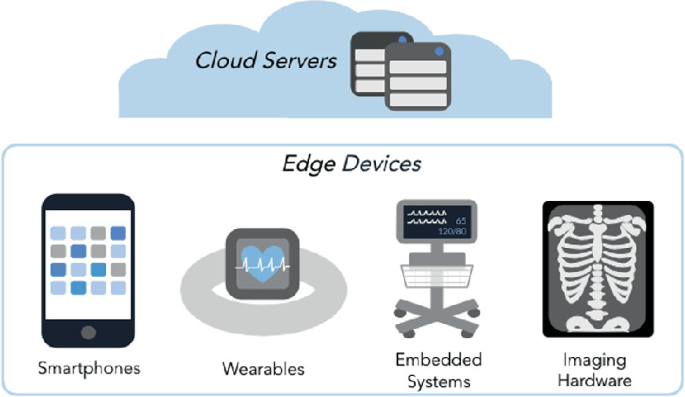
\includegraphics[width=0.8\linewidth]{../img/edge_devices.png}
    \caption{Variants of edge devices (reproduced from \cite{Abid2022EdgeDevices}).}
    \label{fig:edge_devices}
\end{figure}

\noteTime{1:00--1:20. Give one concrete example: phone camera or smart CCTV.}
\end{frame}


% ---------------- Motivation ----------------
\begin{frame}{Motivation: accuracy is not the only constraint}

\begin{itemize}
  \item High benchmark accuracy does not automatically translate to a usable model in production.
  \item In edge/real-time settings (mobile, cameras, robots), inference is constrained by:
  \begin{itemize}
    \item limited throughput for dense ops (e.g., convolutions / attention) on the available accelerator,
    \item memory pressure from weights and feature maps (and the cost of moving them),
    \item power limits that reduce sustained performance.
  \end{itemize}
  \item The goal is \textbf{real-time object detection} with competitive accuracy under these constraints.
  \item This creates a practical trade-off: \textbf{accuracy} vs \textbf{latency} vs \textbf{model size} (and ideally energy).
\end{itemize}

\footnotesize Related survey viewpoint: \cite{sze2017efficient,cheng2017compression}.
\noteTime{1:20--2:20. Use a simple story: “same mAP, different latency”.}
\end{frame}

\begin{frame}{Edge deployment: what “real-time” means}

\begin{itemize}
  \item \textbf{Real-time} means the detector can process a live stream \emph{without visible lag}
        (typically \textbf{15--30 FPS}, depending on the application).
  \item The end-to-end latency is not only the neural network. A full inference pipeline includes:
  \begin{itemize}
    \item input preprocessing (decode / resize / normalise),
    \item model forward pass (backbone + neck + head),
    \item postprocessing (box decoding, NMS),
    \item data movement and I/O (camera capture, memory copies).
  \end{itemize}
  \item Important practical point: \textbf{FLOPs/MACs are only a rough proxy} --- actual latency depends on
        operator support, kernel efficiency, and memory bandwidth on the target device.
\end{itemize}

\noteTime{2:20--3:10. Stress: report end-to-end latency + model-only latency when possible.}
\end{frame}

% ---------------- Aim & Questions ----------------
\begin{frame}{Aim of the work}

\begin{itemize}
  \item The focus is \textbf{real-time object detection on edge devices}, where compute and memory are limited.
  \item I compare efficiency methods that reduce \textbf{inference cost} (compute, memory, bandwidth) while keeping
        detection quality as high as possible.
  \item The main evaluation criteria are \textbf{accuracy} (detection metric), \textbf{latency} (ms / FPS),
        and \textbf{model size}; \textbf{energy} is included when measurement is feasible.
\end{itemize}

\noteTime{3:10--4:00. Say: “accuracy is necessary, but efficiency decides if it can run”.}
\end{frame}


% ---------------- Background: CNNs ----------------
\section{Background: architectures}

\begin{frame}{Convolutional Neural Networks (CNNs): short introduction}

\begin{itemize}
  \item A \textbf{CNN} is a neural network designed for images, where the main operation is the
        \textbf{convolution}: a small learnable filter is applied across the image to detect local patterns.
  \item Stacking convolution layers builds a hierarchy of features:
        \textbf{edges/texture} $\rightarrow$ \textbf{parts} $\rightarrow$ \textbf{objects}.
  \item For object detection, CNNs are typically used as a \textbf{backbone} that produces feature maps,
        which are then processed by a detection head (classification + box regression).
\end{itemize}

\noteTime{4:40--5:10. One sentence transition: “Next: why CNNs are usually efficient on edge”.}
\end{frame}

\begin{frame}{CNNs in vision: why they work well on edge}

\begin{itemize}
  \item CNNs are well-suited for images because they look at \textbf{small local regions} at a time and reuse
        the \textbf{same filter} across the whole image. This makes them efficient and practical to run.
  \item A rough compute proxy for a convolution layer is the number of multiply-accumulate operations:
  \[
    \mathrm{MACs} \approx H'W' \cdot C_{\text{out}} \cdot (k^2 C_{\text{in}}).
  \]
  \item In practice, the \textbf{early layers} (where feature maps are still large) often take most of the time, and
        \textbf{moving data in memory} can be a bottleneck even if the MAC count looks reasonable.
\end{itemize}


\footnotesize See efficiency discussion: \cite{sze2017efficient}.
\noteTime{5:10--6:20. Emphasise: “MACs help compare models, but bandwidth often decides speed”.}
\end{frame}

\begin{frame}{CNN building blocks that matter for efficiency}

\begin{itemize}
  \item \textbf{Residual connections} (ResNet-style) add skip paths that stabilise training, which enables
        deeper backbones without vanishing gradients.
  \item \textbf{Bottleneck blocks} use $1\times1$ convolutions to reduce/expand channels around an expensive
        $3\times3$ convolution, lowering compute while keeping representational power.
  \item \textbf{Downsampling choices} (max-pooling vs strided convolutions) achieve similar spatial reduction,
        but differ in learnability, compute cost, and memory-access patterns.
  \item These blocks define natural \textbf{units for optimisation} later: pruning channels/blocks, or quantising
        weights/activations within them.
\end{itemize}

\footnotesize Background: \cite{lecun2015deep}.
\noteTime{6:20--7:10. Bridge: “compression often operates at the channel/block level”.}
\end{frame}

% ---------------- Background: Transformers ----------------
% --- 1) Intro to Transformers ---
\begin{frame}{Transformers: what they are (high level)}

\begin{itemize}
  \item A \textbf{Transformer} is a neural network that processes a \textbf{sequence of tokens} and builds
        contextual representations for each token.
  \item The key operation is \textbf{self-attention}: each token combines information from other tokens,
        allowing the model to capture long-range dependencies.
  \item In practice, Transformers alternate:
  \begin{itemize}
    \item \textbf{(Multi-head) self-attention} for information mixing,
    \item a \textbf{feed-forward network (MLP)} applied per token.
  \end{itemize}
  \item Unlike CNNs, Transformers do not assume locality by default, which can help modeling global context,
        but often increases computation.
\end{itemize}

\footnotesize Canonical reference: \cite{vaswani2017attention}.
\noteTime{7:10--7:55. Keep it intuitive; details come with ViT.}
\end{frame}

\begin{frame}{Transformer architecture visualisation}

\begin{columns}[T,onlytextwidth]
  \column{0.48\textwidth}
  \centering
  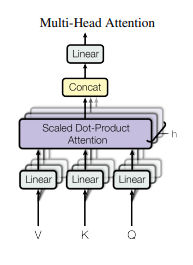
\includegraphics[width=\linewidth,height=0.7\textheight,keepaspectratio]{../img/Multi-Head-Attention.png}
  
  \vspace{1mm}
  {\scriptsize Multi-head self-attention (adapted from \cite{vaswani2017attention}).}

  \column{0.48\textwidth}
  \centering
  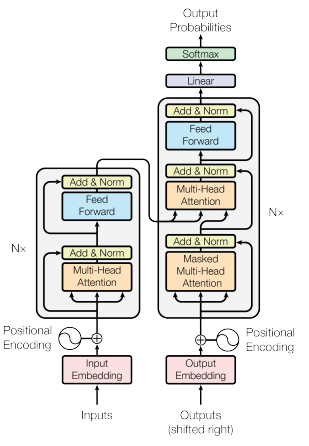
\includegraphics[width=\linewidth,height=0.7\textheight,keepaspectratio]{../img/transformer-architecture.png}
  
  \vspace{1mm}
  {\scriptsize Transformer encoder--decoder overview (adapted from \cite{vaswani2017attention}).}
\end{columns}

\noteTime{9:10--9:50. Briefly point: “attention block + residual + MLP; repeated layers”.}
\end{frame}

% --- 2) Vision Transformers ---
\begin{frame}{Vision Transformers (ViT): applying Transformers to images}

\begin{itemize}
  \item ViT represents an image as a \textbf{sequence of patch tokens}:
        split into $P\times P$ patches and project each patch to an embedding.
  \item The number of tokens grows with resolution:
  \[
    n = \frac{H W}{P^2}.
  \]
  \item After adding positional information, the patch tokens are processed by standard Transformer layers
        (attention + MLP) to produce image features.
  \item For detection, ViT features can be used as a backbone (often combined with CNN-like components).
\end{itemize}

\footnotesize ViT: \cite{dosovitskiy2021vit}.
\noteTime{7:55--8:35. Connect to vision: “patches are like words”.}
\end{frame}

% --- 3) Efficiency implications + common approaches ---
\begin{frame}{Making Transformers efficient for vision (why and how)}

\begin{itemize}
  \item Main cost driver: global attention compares all token pairs $\Rightarrow$ \textbf{quadratic cost}
        $O(n^2)$ in the number of tokens, which grows quickly with image resolution.
  \item Common efficiency ideas in vision transformers:
  \begin{itemize}
    \item \textbf{Local / windowed attention} (attend within neighborhoods instead of globally),
    \item \textbf{Hierarchical representations} (downsample tokens across stages, similar to CNN feature pyramids),
    \item \textbf{Efficient attention variants} (approximate/sparse attention, linear-time forms),
    \item \textbf{Hybrid models} (CNN stem or mixed blocks) to keep locality where it helps.
  \end{itemize}
  \item Practical takeaway for edge: CNNs are often simpler to deploy efficiently, while ViTs may need
        these design choices (plus quantisation/pruning) to meet real-time constraints.
\end{itemize}

\noteTime{8:35--9:10. Message: “attention is powerful, but needs efficiency tricks at high resolution”.}
\end{frame}



% ---------------- Toolbox: Quantisation ----------------
\section{Efficiency toolbox}

\begin{frame}{Numeric precision in inference (FP32, FP16, INT8)}

\begin{itemize}
  \item Neural networks store \textbf{weights} and compute \textbf{activations} using finite-precision numbers.
  \item \textbf{FP32} (32-bit float) is the default in training: high precision, but larger memory and slower inference.
  \item \textbf{FP16} (16-bit float) is common for faster inference/training on GPUs: similar accuracy in many cases.
  \item \textbf{INT8} (8-bit integer) is widely used for edge inference: much smaller tensors and potentially faster kernels.
  \item Lower precision saves memory/bandwidth, but can introduce \textbf{quantisation error} that may reduce accuracy.
\end{itemize}

\noteTime{9:10--9:40. One line: “lower bits = cheaper inference, but we must control accuracy drop”.}
\end{frame}

\begin{frame}{Quantisation: idea and why it helps}

\begin{itemize}
  \item \textbf{Quantisation} replaces FP32 computations with lower precision (typically \textbf{FP16} or \textbf{INT8})
        for weights and/or activations.
  \item A common approach is an affine mapping with a scale $s$ and zero-point $z$:
  \[
    x_q = \mathrm{clip}\left(\left\lfloor \frac{x}{s}\right\rceil + z, q_{\min}, q_{\max}\right),
    \qquad
    \hat{x} = s(x_q - z).
  \]
  \item In practice, the main benefits are:
  \begin{itemize}
    \item \textbf{smaller model} and lower memory bandwidth (especially for activations),
    \item \textbf{faster inference} when the runtime/device has efficient INT8 kernels.
  \end{itemize}
\end{itemize}

\footnotesize Surveys: \cite{gholami2021quant,sze2017efficient}.
\noteTime{9:40--10:30. Emphasise: “INT8 speedup depends on kernel support + memory bandwidth”.}
\end{frame}


\begin{frame}{PTQ vs QAT: two ways to get an INT8 model}

\begin{columns}[T,onlytextwidth]
\column{0.48\textwidth}
\textbf{Post-training quantisation (PTQ)}
\begin{itemize}
  \item Start from a trained FP32 model and quantise it after training.
  \item Use a small calibration set to estimate activation ranges.
  \item Very fast to apply, but accuracy can drop (often more noticeable in detection).
\end{itemize}

\column{0.48\textwidth}
\textbf{Quantisation-aware training (QAT)}
\begin{itemize}
  \item Train with \textbf{fake quantisation} so the model learns to be robust to INT8 rounding/clipping.
  \item Typically achieves higher INT8 accuracy than PTQ.
  \item Costs additional training effort and careful tuning.
\end{itemize}
\end{columns}

\footnotesize Reference survey: \cite{gholami2021quant}.
\noteTime{10:30--11:40. Framing: “PTQ = quick baseline; QAT = best accuracy when INT8 matters”.}
\end{frame}


% ---------------- Toolbox: Pruning ----------------
\begin{frame}{Pruning: remove redundancy in the network}

\begin{itemize}
  \item \textbf{Pruning} removes parameters that contribute little to the final prediction, aiming to keep accuracy
        while reducing inference cost.
  \item A simple view is applying a binary mask $m$ to parameters:
  \[
    \theta' = m \odot \theta.
  \]
  \item Two common types (with different practical outcomes):
  \begin{itemize}
    \item \textbf{Unstructured pruning:} removes individual weights $\Rightarrow$ high sparsity, but the computation becomes irregular.
    \item \textbf{Structured pruning:} removes whole channels/filters/blocks $\Rightarrow$ a smaller \emph{dense} model that is easier to accelerate.
  \end{itemize}
  \item For real-time edge inference, \textbf{structured pruning is often more useful}, because it reliably reduces
        tensor sizes and translates to lower latency.
\end{itemize}

\footnotesize Classic: \cite{han2016deepcompression}; survey: \cite{cheng2017compression}.
\noteTime{11:40--12:50. Key point: “sparsity does not guarantee speed unless sparse kernels are used”.}
\end{frame}

% ---------------- Toolbox: Distillation ----------------
\begin{frame}{Knowledge distillation: teacher $\rightarrow$ student}

\begin{itemize}
  \item \textbf{Goal:} train a smaller \emph{student} model to match a stronger \emph{teacher} while keeping good accuracy.
  \item The student learns from two sources:
  \begin{itemize}
    \item \textbf{hard targets} (ground-truth labels),
    \item \textbf{soft targets} (teacher predictions), which contain extra information about class similarities.
  \end{itemize}
  \item Soft targets are usually produced with temperature $\tau$:
  \[
    p_T(\tau)=\mathrm{softmax}\!\left(\frac{z_T}{\tau}\right),\qquad
    p_S(\tau)=\mathrm{softmax}\!\left(\frac{z_S}{\tau}\right).
  \]
  \item Training loss typically combines the standard supervised loss with a \textbf{distillation loss}
        (often KL divergence between $p_T$ and $p_S$).
\end{itemize}

\footnotesize Distillation: \cite{hinton2015distill}.
\noteTime{12:50--14:00. Message: “teacher provides richer targets than one-hot labels”.}
\end{frame}

\begin{frame}{Distillation in object detection: what changes}

\begin{itemize}
  \item Object detection is not only classification: the output is \textbf{structured}
        (class scores + box regression, sometimes dense maps).
  \item Therefore, distillation can be applied at multiple levels:
  \begin{itemize}
    \item \textbf{classification logits/scores} (confidence distribution),
    \item \textbf{box regression outputs} (localisation),
    \item \textbf{intermediate features} (backbone/neck representations),
    \item \textbf{dense predictions} (e.g., heatmaps or feature pyramids, depending on the detector).
  \end{itemize}
  \item In an efficiency pipeline, distillation is often a \textbf{recovery step}:
        after pruning or INT8 quantisation, it helps the student regain lost accuracy.
\end{itemize}

\noteTime{14:00--15:00. Example line: “teacher stabilises ranking and localisation after compression”.}
\end{frame}

% ---------------- Toolbox: NAS ----------------
\begin{frame}{Hardware-aware NAS / efficient-by-design models}

\begin{itemize}
  \item Instead of compressing a fixed network, \textbf{neural architecture search (NAS)} tries to find an
        architecture $\alpha$ that is accurate \emph{and} meets a deployment budget:
  \[
    \max_{\alpha \in \mathcal{A}} \mathrm{Acc}(\alpha)
    \quad \text{s.t.}\quad
    \mathrm{Cost}(\alpha)\le C_{\max}.
  \]
  \item The key is that \textbf{Cost} should reflect the \emph{target runtime/device} (e.g., measured latency,
        memory footprint, sometimes energy), not only FLOPs.
  \item In practice (especially with limited time/compute), a common workflow is:
  \begin{itemize}
    \item start from an efficient baseline architecture,
    \item restrict the search/tuning to a small design space (e.g., widths, depths, kernel sizes),
    \item optionally tune only parts of the detector (neck/head),
    \item use a latency predictor or on-device measurements to guide choices.
  \end{itemize}
  \item Takeaway: \textbf{NAS designs efficiency in}, while pruning/quantisation \textbf{shrink an existing model}.
\end{itemize}

\footnotesize Example: \cite{cai2019proxylessnas}.
\noteTime{15:00--16:10. Emphasise the contrast: “design vs compression”.}
\end{frame}

% ---------------- Combining methods ----------------
\begin{frame}{Compression pipelines: why combinations matter}

\begin{itemize}
  \item These techniques improve efficiency in \textbf{different ways}, so combining them is often better than using
        only one method:
  \begin{itemize}
    \item \textbf{Pruning} reduces model capacity and tensor sizes $\rightarrow$ fewer operations in a smaller dense network.
    \item \textbf{Quantisation} reduces numerical precision $\rightarrow$ fewer bits to move/store and faster INT8 kernels (when supported).
    \item \textbf{Distillation} transfers knowledge from a strong teacher $\rightarrow$ helps recover accuracy after compression.
  \end{itemize}

  \item A practical pipeline for real-time detection can look like:
  \begin{enumerate}
    \item choose an efficient baseline detector,
    \item apply \textbf{structured pruning} to meet the latency budget,
    \item apply \textbf{QAT} to obtain a robust INT8 model,
    \item \textbf{distill} from a stronger teacher to regain lost accuracy.
  \end{enumerate}

  \item Important caveat: the final outcome depends strongly on the \textbf{hardware and runtime stack},
        so results should be validated on the target setup.
\end{itemize}

\noteTime{16:10--17:30. Bridge: “this motivates the evaluation protocol and device benchmarking”.}
\end{frame}

\section{Evaluation}

\begin{frame}{Evaluation protocol for fair comparison}

\begin{itemize}
  \item \textbf{Goal:} compare methods fairly under a realistic deployment pipeline, not only in theory.
  \item Keep the setup fixed across experiments:
  \begin{itemize}
    \item the same input resolution(s), preprocessing, and postprocessing (especially NMS),
    \item the same dataset splits, augmentation policy, and training budget.
  \end{itemize}
  \item Report a consistent set of metrics:
  \begin{itemize}
    \item \textbf{accuracy:} mAP@[.5:.95] (COCO-style) or the dataset-appropriate detection metric,
    \item \textbf{latency:} end-to-end and model-only time (ms / FPS), with warm-up vs cold-start noted,
    \item \textbf{model size:} on-disk weights and (if possible) peak runtime memory.
  \end{itemize}
  \item Benchmark using the \textbf{intended inference runtime} (e.g., TFLite / TensorRT / ONNX Runtime),
        because results can change significantly across stacks.
\end{itemize}

\noteTime{17:30--18:40. Mention: “same training budget, same resolution, same NMS”.}
\end{frame}


\begin{frame}{Deployment stack matters more than people expect}

\begin{itemize}
  \item Even with identical weights, the \textbf{observed latency} can differ depending on the deployment stack.
  \item Differences often come from:
  \begin{itemize}
    \item operator coverage (e.g., whether INT8 conv/attention is actually supported),
    \item kernel implementations and fusions (what gets fused vs executed separately),
    \item memory layout and bandwidth effects (activation movement can dominate),
    \item backend selection (CPU vs GPU vs NPU / delegate choice).
  \end{itemize}
\end{itemize}

\noteTime{18:40--19:40. Tie to RQ6: “measure on target stack, not only FLOPs”.}
\end{frame}


\begin{frame}{Energy measurement}

\begin{itemize}
  \item On battery-powered platforms, \textbf{energy per inference} can be as important as accuracy or latency.
  \item Practical measurement options (depending on the device):
  \begin{itemize}
    \item OS-level counters / onboard sensors (when available),
    \item external power meter (e.g., for phones or SBCs),
    \item steady-state measurement during repeated inference to estimate average power.
  \end{itemize}
  \item Report both:
  \begin{itemize}
    \item \textbf{power} in watts (W) during inference,
    \item \textbf{energy per frame} (J/frame) = average power $\times$ inference latency.
  \end{itemize}
\end{itemize}

\noteTime{19:40--20:30. Keep it framed as “nice-to-have if feasible”.}
\end{frame}

\begin{frame}{Future work}

\begin{itemize}
  \item This area evolves quickly: new architectures and compression methods appear every year, and results
        can change as runtimes and hardware improve.
  \item \textbf{Lower-bit quantisation:} beyond INT8, current research increasingly explores \textbf{INT4} (and mixed precision)
        to further reduce memory and bandwidth, with new techniques to stabilise accuracy.
  \item \textbf{New efficient architectures:} vision backbones (CNN/Transformer/hybrid) continue to improve,
        especially designs targeting latency and memory on specific hardware.
  \item \textbf{Better end-to-end pipelines:} further optimisation of preprocessing, postprocessing (e.g., NMS),
        and runtime-level fusions can yield speedups without changing the core model.
  \item These directions are natural candidates for extension in the final thesis and experimental work.
\end{itemize}

\noteTime{20:30--21:10. Emphasise: “this thesis evaluates a snapshot; the toolbox keeps expanding”.}
\end{frame}


% ---------------- Plan / Next steps ----------------
\section{Wrap-up}


\begin{frame}{Key takeaways}
\begin{itemize}
  \item Edge deployment is a \textbf{systems problem}: model + hardware + runtime.
  \item CNNs are still strong for edge; transformers need careful efficiency design.
  \item Best results often come from \textbf{method combinations} (prune + INT8 + distill).
  \item Measuring on the target stack is essential for answering the research questions.
\end{itemize}
\noteTime{21:30--22:20. Leave 1--2 minutes for questions.}
\end{frame}


% ---------------- References ----------------
\begin{frame}[allowframebreaks]{References}
\printbibliography
\end{frame}

\begin{frame}[standout]
Thank you for your attention!
\noteTime{22:20--24:00. Discussion buffer.}
\end{frame}



\end{document}
